\documentclass[preprint,authoryear,number]{elsarticle}
\usepackage{setspace}
\setlength{\parskip}{0.5em}
\usepackage[utf8]{inputenc}
\usepackage[T1]{fontenc}
\usepackage{amsmath,amssymb}
\usepackage{graphicx}
\usepackage{booktabs}
\usepackage{multirow}
\usepackage{xcolor}
\usepackage{hyperref}
\usepackage{siunitx}
\usepackage{lineno}
\usepackage{natbib}
\modulolinenumbers[5]
\linenumbers

% Placeholder for figures not yet produced (F2, F3, F5, F6): see paper/manuscript.workbook.md
\newcommand{\figplaceholder}[1]{\fbox{\parbox[c][5cm][c]{0.9\textwidth}{\centering\small\textit{Figure in preparation: #1}}}}

\journal{(venue to be decided)}

\begin{document}
\begin{frontmatter}

\title{Negative-set design, not the search algorithm, determines the transferability of Sentinel-2 hydrothermal alteration indices}

\author[usach]{Francisco Parra~O.\corref{cor1}}
\ead{francisco.parra.o@usach.cl}
\cortext[cor1]{Corresponding author}
\author[dim]{Gonzalo R\'ios}
\author[uoh,systemix,cgr,cmm,inta]{Mauricio Latorre}

\address[usach]{Universidad de Santiago de Chile (USACH), Santiago, Chile}
\address[dim]{Departamento de Ingenier\'ia Matem\'atica, Facultad de Ciencias F\'isicas y Matem\'aticas, Universidad de Chile, Santiago, Chile}
\address[uoh]{Laboratorio de Bioingenier\'ia, Instituto de Ciencias de la Ingenier\'ia, Universidad de O'Higgins, Libertador Bernardo O'Higgins 611, Rancagua, Chile}
\address[systemix]{Centro de Biolog\'ia de Sistemas para el Estudio de Comunidades Extrem\'ofilas de Relaves Mineros (SYSTEMIX), Universidad de O'Higgins, Rancagua, Chile}
\address[cgr]{Millennium Institute Center for Genome Regulation, Santiago 8320165, Chile}
\address[cmm]{Center for Mathematical Modeling, University of Chile, Beauchef 851, Santiago, Chile}
\address[inta]{Laboratorio de Bioinform\'atica y Expresi\'on G\'enica, INTA, Universidad de Chile, El L\'ibano 5524, Macul, Santiago, Chile}

\begin{abstract}
Spectral indices for mapping hydrothermal alteration with Sentinel-2 are routinely evaluated against easy negatives: unaltered rock sampled far from the alteration they are meant to detect. Under that protocol almost any new index outperforms the classical clay ratio (B11/B12), yet the gain rarely survives a change of site. We show that what decides whether an index transfers is the design of the negative set, not the algorithm that searches for the index. We build hard negatives from the host-rock ring \SIrange{300}{2000}{\meter} around every mapped alteration polygon, plus spectral distractors (salt flats, snow, shadow, vegetation, alluvium), and select indices in Chile's Atacama Region under a \SI{10}{\kilo\meter} spatial-block split. Instead of a stochastic search, we enumerate the complete family of band-ratio products and normalised differences up to five factors (452{,}706 expressions), which yields the exact Pareto front of accuracy versus complexity and removes the search as a source of variation. With the same family, selection against distant negatives or against the ring alone picks indices that fail to transfer; selection against the ring plus distractors picks the four-ratio index B02$\cdot$B8A$^2\cdot$B12/(B03$\cdot$B04$\cdot$B11$^2$). At two sites never used for selection it outperforms the clay ratio by 0.11--0.12 AUC in Chile's Coquimbo Region and by 0.06--0.09 at Cuprite, Nevada, with block-bootstrap confidence intervals excluding zero, and it lowers the mean false-positive rate on distractors from 55\% to 10\% and from 28\% to 5\%. The index sits within 0.02 AUC of a logistic model over all log-ratios and transfers better than random forests trained on the same data. Its gain is in specificity: against adjacent host rock alone the clay ratio is better at the selection site, and the index is stable across years but degrades in the opposite season. The negative-set design and the enumeration are sensor-agnostic; code and extracted pixels are public.
\end{abstract}

\begin{keyword}
Hydrothermal alteration \sep Sentinel-2 \sep Spectral indices \sep Negative sampling \sep Exhaustive enumeration \sep Cross-site transfer
\end{keyword}
\end{frontmatter}

%% ============================================================
\section{Introduction}
\label{sec:intro}

Multispectral mapping of hydrothermal alteration rests on band ratios chosen from the physics of mineral absorption. Hydroxyl-bearing clays, micas and sulfates absorb near \SI{2.2}{\micro\meter}, ferric oxides absorb near \SI{0.9}{\micro\meter} and reflect strongly in the red, and ratios placed across these features have guided exploration since the Landsat era \citep{Sabins1999}. Indices designed for the six shortwave infrared (SWIR) bands of ASTER \citep{Ninomiya2005,Mars2006,Mars2010} were later adapted to Sentinel-2, which offers only two SWIR bands but finer spatial resolution, frequent revisits and free global coverage \citep{vanderMeer2014,vanderWerff2016,Pour2018}. The ratio B11/B12, commonly called the clay ratio, is the Sentinel-2 workhorse of this family.

How these indices are evaluated matters as much as how they are designed. The usual protocol compares pixels inside mapped alteration with unaltered pixels sampled elsewhere: in another lithology, in another landscape, often kilometres away. Such a test measures whether an index separates landscapes, not whether it separates altered rock from the rock that hosts it. It also omits the surfaces that are known to mimic alteration in arid terrain, such as evaporites, bright alluvium, topographic shadow and residual snow. An index that wins under this protocol may simply be a better landscape classifier, and its advantage is expected to vanish at a new site where the background differs. The same concern is familiar in species distribution modelling, where the choice of pseudo-absences changes model performance and transfer \citep{Phillips2009,BarbetMassin2012}, and in mineral prospectivity mapping, where random negative samples have been shown to affect the resulting maps \citep{Zuo2020,Zhang2025}. It has received little attention for spectral indices.

When indices are searched for automatically rather than designed by hand, a second source of variation appears. Genetic programming has been used to evolve spectral expressions for mineral identification \citep{Ross2005} and for vegetation \citep{Momm2011}, and symbolic regression has produced compact Sentinel-2 indices validated across independent regions \citep{Chrysostomou2026}. These searches are stochastic: different runs return different expressions, and the result is not compared with the optimum of the space being searched. In symbolic regression, exhaustive enumeration has shown that genetic programming visits only a small fraction of the distinct expressions of a given size \citep{Bartlett2024,Kronberger2024}. Enumerations of band pairs are routine in hyperspectral vegetation studies \citep{Thenkabail2000}, and a recent library of scale-invariant features for Sentinel-2 combines enumeration with a pre-filter and spatial cross-validation \citep{Lotfi2026}. For alteration, exhaustive treatments of band ratios exist only as unsupervised transformations \citep{Askari2018}.

In this study we separate the two factors. First, we build a hard negative set made of the host rock that surrounds each mapped alteration polygon and of the spectral distractors of the region. Second, we enumerate every member of a closed family of indices, so that the search algorithm is no longer a variable: the best index of the family under a given criterion is known exactly. We then fix a transfer rule and test the selected index at two sites that never enter the selection, one in the same metallogenic belt and one on another continent.

We ask three questions. (RQ1) Does the negative set used for selection change which index wins and whether it transfers? (RQ2) Does the optimum of the family transfer to independent sites, and how far is it from a linear model over all log-ratios and from machine-learning classifiers trained on the same data? (RQ3) Where does the selected index fail?

%% ============================================================
\section{Study areas and data}
\label{sec:data}

\subsection{Selection site: Atacama Region, Chile}

Indices are selected in the Maricunga metallogenic belt of Chile's Atacama Region (\ang{26}--\ang{28}\,S, \ang{68.4}--\ang{69.5}\,W; Fig.~\ref{fig:study_area}). The belt hosts Oligocene--Miocene porphyry Au--Cu and epithermal systems emplaced in andesitic to dacitic volcanic sequences at \SIrange{3500}{5000}{\meter} elevation \citep{Sillitoe1991,Vila1991}. Alteration is mapped in the \emph{Atlas Metal\'ifero de la III Regi\'on} of the Chilean geological survey (SERNAGEOMIN) at 1:100{,}000, as 636 polygons: 92 assigned to alteration classes and 544 labelled as undifferentiated hydrothermal alteration. We treat all of them as altered. The region also offers, within a single Sentinel-2 composite, the main surfaces that are confused with alteration in the Andes: salt flats, bright alluvium, snow, shadow on steep slopes and sparse vegetation, which makes it a demanding site for selection.

\subsection{Test site 1: Coquimbo Region, Chile}

The first test site lies in Chile's Coquimbo Region (\ang{30}--\ang{31}\,S), about \SI{300}{\kilo\meter} south of the selection site, in the same Andean metallogenic context but with different host lithologies and alteration geometries. Alteration polygons (147) come from four SERNAGEOMIN geological sheets (Vicu\~na--Pichasca, Andacollo--Puerto Aldea, Ovalle--Pe\~nablanca and Monte Patria--El Maqui).

\subsection{Test site 2: Cuprite, Nevada, USA}

The second test site is the Cuprite mining district, Nevada (\ang{37.5}\,N, \ang{117.2}\,W), the most widely used benchmark for spectral mapping of alteration \citep{Swayze2014}. Its late Miocene advanced argillic and silicic alteration formed in a Basin and Range extensional setting, which differs from the Andean compressional belt in tectonics, age and climate. Ground truth is the USGS map of hydrothermal alteration of the southwestern United States \citep{Rockwell2017}, derived from ASTER with the Tetracorder expert system. Because this map comes from spectral analysis rather than field mapping at 1:100{,}000, its labels are expected to be cleaner than the Chilean ones; we use that contrast in the Discussion. The mapped alteration extends well beyond the classical Cuprite window (two thirds of the mapped area within \SI{15}{\kilo\meter} lies outside it, mainly towards Goldfield), so all negative sampling at this site uses the enlarged map.

\subsection{Sentinel-2 composites and samples}

We used Sentinel-2 Level-2A surface reflectance (collection S2\_SR\_HARMONIZED) in Google Earth Engine \citep{Gorelick2017}. Each site has one median composite of the dry season of 2024 (Table~\ref{tab:composites}), scaled to reflectance and analysed at \SI{20}{\meter}, the native resolution of B11 and B12. Ten bands were retained: B02--B07, B08, B8A, B11 and B12. Positive pixels were sampled inside the mapped alteration of each site with their coordinates, so that every pixel can be assigned to a spatial block (Section~\ref{sec:split}). Because Earth Engine composites are not guaranteed to be bit-reproducible over time, the extracted pixel tables, not the composites, are the reference data for every number in this paper; resampling the base composites at the time of writing reproduced the stored values (median relative difference 0).

\begin{table}[ht]
\centering
\caption{Sentinel-2 composites and positive samples per site.}
\label{tab:composites}
\small
\begin{tabular}{llrrr}
\toprule
Site & Period (2024) & Cloud limit & Scenes & Positive pixels \\
\midrule
Atacama (selection) & Jan--Mar & 20\% & 825 & 8{,}000 (460 polygons) \\
Coquimbo (test 1) & Jan--Mar & 20\% & 64 & 7{,}050 \\
Cuprite (test 2) & Jun--Sep & 15\% & 118 & 3{,}760 (182 mapped blobs) \\
\bottomrule
\end{tabular}
\end{table}

\begin{figure*}[ht]
\centering
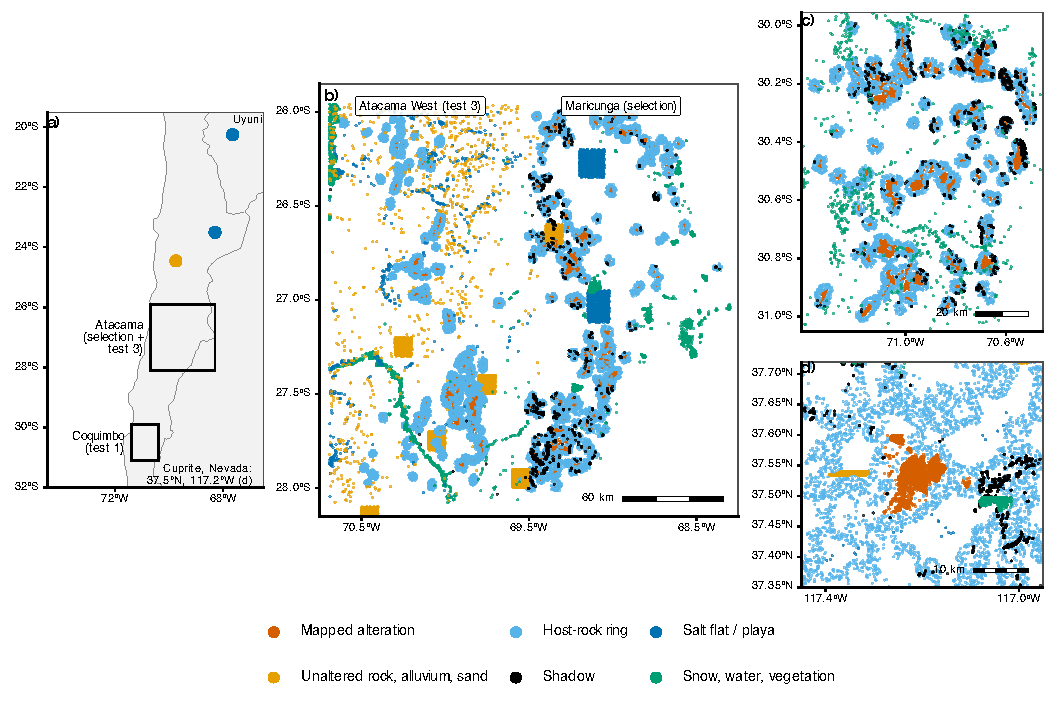
\includegraphics[width=\textwidth]{../figures/v2/fig1_study_areas.pdf}
\caption{Study areas and hard negative set. (a)~Selection site (Atacama Region) and first test site (Coquimbo Region), Chile, with the location of the distant distractor boxes (Salar de Uyuni, Salar de Atacama and aeolian sand). (b)~Atacama: mapped alteration of the \emph{Atlas Metal\'ifero de la III Regi\'on} and the sampled negatives (host-rock ring \SIrange{0.3}{2}{\kilo\meter} from mapped alteration, salt flats, unaltered lithologies, snow, water, vegetation and shadow). (c)~Coquimbo: mapped alteration and sampled negatives. (d)~Cuprite, Nevada: positive samples inside the USGS alteration map and sampled negatives; the ring extends over the enlarged map. Map lines delineate study areas and do not necessarily depict accepted national boundaries.}
\label{fig:study_area}
\end{figure*}

%% ============================================================
\section{Methods}
\label{sec:methods}

\subsection{Hard negative set}
\label{sec:negatives}

The negative set has two parts. The first is a \emph{host-rock ring}: the band between \SI{300}{\meter} and \SI{2}{\kilo\meter} from the union of all mapped alteration polygons of a site. The inner limit leaves a margin for the positional error of 1:100{,}000 mapping; the outer limit keeps the ring in the same lithological units and landscape as the alteration it surrounds. Ring pixels are therefore the hardest negatives that the maps allow: rock of the same district that the geologist did not map as altered. At Cuprite the ring is drawn on the enlarged USGS map, so that it never falls on unmapped ground.

The second part is a set of \emph{distractors} defined by spectral and topographic criteria and sampled outside a \SI{300}{\meter} buffer of mapped alteration (Table~\ref{tab:negatives}). In Atacama they include four salt flats, aeolian sand, snow (normalised difference snow index above 0.4 and elevation above \SI{5000}{\meter}), shadow (slope above \ang{20} and low hillshade), vegetation (NDVI above 0.3), open water (NDWI above 0.2) and six unaltered lithologies. In Coquimbo the distractors are shadow and vegetation; at Cuprite they are shadow, vegetation, water, playas (slope below \ang{2}, red reflectance above 0.30, NDVI below 0.10) and alluvium, sampled more than \SI{2}{\kilo\meter} from mapped alteration. Vegetation and water are routinely masked with NDVI and NDWI before alteration mapping, so they receive zero weight in selection and are excluded from the evaluation sets that combine ring and distractors; their false-positive rates are still reported.

For comparison we keep the negatives of a conventional design: 8{,}000 pixels from four boxes about \SI{25}{\kilo\meter} outside the alteration zone, within the same geological province. We call them \emph{distant negatives}.

\begin{table}[ht]
\centering
\caption{Negative groups and number of pixels per site.}
\label{tab:negatives}
\small
\resizebox{\textwidth}{!}{%
\begin{tabular}{llrrr}
\toprule
Group & Criterion & Atacama & Coquimbo & Cuprite \\
\midrule
Host-rock ring & \SIrange{0.3}{2}{\kilo\meter} from mapped alteration & 8{,}000 & 7{,}000 & 4{,}000 \\
Shadow & slope $>\ang{20}$, low hillshade & 1{,}500 & 1{,}500 & 1{,}500 \\
Salt flats & four named salars & 3{,}200 & -- & -- \\
Playa & flat, bright, NDVI $<0.10$ & -- & -- & 800 \\
Alluvium / sand & flat, NDVI $<0.15$ / aeolian sand & 800 & -- & 800 \\
Snow & NDSI $>0.4$, $>\SI{5000}{\meter}$ & 800 & -- & -- \\
Unaltered lithologies & six mapped units & 4{,}712 & -- & -- \\
Vegetation$^{a}$ & NDVI $>0.3$ & 800 & 800 & 800 \\
Water$^{a}$ & NDWI $>0.2$ & 800 & -- & 520 \\
\bottomrule
\multicolumn{5}{l}{\footnotesize $^{a}$Weight 0 in selection; excluded from ``ring + distractors'' evaluation sets.}
\end{tabular}}
\end{table}

\subsection{Index family and exhaustive enumeration}
\label{sec:enumeration}

We consider indices that are products of powers of band reflectances,
\begin{equation}
I(\mathbf{c}) = \prod_{b} B_b^{\,c_b}, \qquad \log I = \sum_{b} c_b \log B_b, \qquad \sum_b c_b = 0,
\label{eq:family}
\end{equation}
where $\mathbf{c}$ is an integer vector over the ten bands. The constraint $\sum_b c_b = 0$ makes every index invariant to a multiplicative change of brightness, such as that produced by illumination or topography. We define the complexity $m = \lVert \mathbf{c} \rVert_1 / 2$ as the number of ratio factors: $m = 1$ gives simple ratios such as B11/B12, $m = 2$ gives products or quotients of two ratios, and so on.

The family is complete for the purpose of a threshold-free evaluation. AUC depends only on the ranking of pixels, and the normalised difference $(B_i - B_j)/(B_i + B_j)$ equals $\tanh\left(\tfrac{1}{2}\log(B_i/B_j)\right)$, a monotone function of the ratio; it is therefore the same index as $B_i/B_j$. For the same reason $k\mathbf{c}$ and $\mathbf{c}$ are the same index, and $\mathbf{c}$ and $-\mathbf{c}$ differ only in orientation. We enumerate every vector that is primitive (coefficients without a common divisor), canonical in sign and has disjoint positive and negative supports, for $m \le 5$: 45, 990, 11{,}220, 74{,}745 and 365{,}706 expressions for $m = 1, \dots, 5$, or 452{,}706 in total. In log space each index is a linear projection of the log-reflectances, so the whole family is scored with matrix products; $m \le 4$ (87{,}000 expressions) takes about 12 minutes and $m \le 5$ about an hour on a laptop CPU.

Because every expression is scored, the best index at each complexity is known exactly, and so is the Pareto front of selection accuracy versus complexity. There is no stochastic search and no dependence on a random seed. We report the symbolic-regression formula of our earlier work as a baseline (Section~\ref{sec:baselines}) but do not rerun a stochastic search: within this family it cannot find an expression that the enumeration has not already scored.

\subsection{Selection criterion and spatial split}
\label{sec:split}

Indices are ranked by a weighted AUC computed on the selection half of the Atacama data. Let $P$ be the positive pixels and $N_g$ the negative pixels of group $g$. The criterion is
\begin{equation}
\mathrm{AUC}_w(I) = \sum_g w_g \, \Pr\left[I(p) > I(n)\right], \quad p \in P,\ n \in N_g,
\label{eq:wauc}
\end{equation}
with ties counted as one half. The host-rock ring carries half of the weight and the remaining half is shared equally among the distractor groups, each group weighted as a whole regardless of its size; vegetation and water have $w_g = 0$. The orientation of each index is the one that gives $\mathrm{AUC}_w \ge 0.5$.

To answer RQ1 we repeat the selection with two other criteria on the same family: positives against the host-rock ring only, and positives against distant negatives. All three selections use only Atacama pixels.

The Atacama data are split into a selection half and a held-out half by spatial blocks of \SI{10}{\kilo\meter} for positives and ring pixels and of \SI{2}{\kilo\meter} for the distractor boxes, which are about \SI{10}{\kilo\meter} wide; whole blocks go to one side \citep{Roberts2017,Meyer2022}. Selecting among 87{,}000 expressions with the same pixels used to report accuracy would bias the reported AUC upwards \citep{Ambroise2002}, so Atacama accuracy is always reported on the held-out half. As a sensitivity analysis we repeat the selection with splits by pixel and by alteration polygon.

\subsection{Transfer gate}
\label{sec:gate}

An index is considered to transfer to a test site if it meets three conditions at that site: (i) its AUC against the host-rock ring exceeds that of the clay ratio by at least 0.03; (ii) the same holds against the ring plus distractors; and (iii) its mean false-positive rate on distractors, at the threshold that maximises Youden's $J$ on the selection set, is not higher than that of the clay ratio. The rule was fixed during a pilot study that used the ring-only criterion. That pilot failed the rule in Coquimbo, which led us to the ring-plus-distractors criterion; Coquimbo had therefore been inspected before the final criterion was chosen, although never used to score expressions. Cuprite was added afterwards, with the rule and the criterion already fixed, and is the cleaner of the two tests.

\subsection{Baselines and uncertainty}
\label{sec:baselines}

We compare the selected index with four closed-form indices: the clay ratio B11/B12, the ferric ratio B04/B02, the best index of complexity $m = 2$, and the binary symbolic-regression formula $(\sqrt{B12} - B11)^2$ of our earlier work. As a ceiling for the family we fit a logistic regression on the nine log-ratios $\log(B_b/B08)$, which is the continuous relaxation of Eq.~\ref{eq:family}. As machine-learning baselines we train random forests (300 trees, minimum leaf size 5) on the ten raw bands and on the nine log-ratios. All models are trained on the Atacama selection half with the weights of Eq.~\ref{eq:wauc} and never see the test sites.

Confidence intervals come from a block bootstrap with 1{,}000 replicates, in which positives and negatives are resampled jointly by spatial blocks of \SI{10}{\kilo\meter} in Chile and \SI{2}{\kilo\meter} at Cuprite, whose alteration spans about \SI{16}{\kilo\meter}. Differences in AUC with respect to the clay ratio are computed within each replicate. Besides AUC we report the true-positive rate at false-positive rates of 5, 10 and 20\%, the false-positive rate at a true-positive rate of 80\%, and the false-positive rate of every negative group at the Youden threshold of the selection set.

\subsection{Temporal stability}
\label{sec:temporal}

The selected index must not depend on one composite. We resampled every stored pixel on two alternative composites per site: the same season one year earlier (2023), and the opposite season of 2024 (June--September in Chile, March--May at Cuprite). Labels, sets and index orientation are unchanged; only reflectances change. We report the AUC of each index on each composite and the Spearman correlation of index values between the base and the alternative composites.

%% ============================================================
\section{Results}
\label{sec:results}

\subsection{RQ1: the selection criterion decides the winner}
\label{sec:rq1}

The three criteria select three different indices from the same 87{,}000 expressions, and only one of them transfers (Table~\ref{tab:criteria}). Selection against distant negatives picks B02$\cdot$B05$\cdot$B8A$\cdot$B12/(B03$\cdot$B04$^2\cdot$B11). It beats the clay ratio in Coquimbo by 0.06--0.07 AUC but not at Cuprite (+0.02 and +0.03), and its selection ranking is unrelated to performance in Coquimbo: across the family, the Spearman correlation between selection AUC and Coquimbo AUC is $-0.10$. Its Coquimbo result is therefore not something the criterion could have predicted. Selection against the host-rock ring alone picks B02$\cdot$B04$\cdot$B12$^2$/(B03$^2\cdot$B11$^2$), which fails at both sites (gains of 0.01--0.03). Selection against the ring plus distractors picks B02$\cdot$B8A$^2\cdot$B12/(B03$\cdot$B04$\cdot$B11$^2$), which passes the AUC conditions at both sites, and its ranking is the most consistent with the test sites ($\rho = 0.53$ with Coquimbo and $0.66$ with Cuprite, Fig.~\ref{fig:scatter}).

The false-positive rates tell the same story. At the Youden threshold of the final selection set, the ring-only winner flags 42\% of the Coquimbo ring and 46\% of its distractors, close to the clay ratio (54\% and 55\%). The distant-negative winner flags few negatives in Coquimbo (3\% and 10\%) but also few positives (recall 17\%), because its threshold no longer means the same thing at a new site. The ring-plus-distractors winner flags 24\% of the ring and 10\% of the distractors while recovering 58\% of the positives.

\begin{table*}[ht]
\centering
\caption{Winner of the same 87{,}000-expression family under three selection criteria, evaluated on the same test sets. $\Delta$ = AUC gain over the clay ratio (ring / ring + distractors). $\rho$ = Spearman correlation, across the family, between selection AUC and test AUC (ring + distractors). Gate = AUC conditions (i) and (ii) of Section~\ref{sec:gate}.}
\label{tab:criteria}
\resizebox{\textwidth}{!}{%
\begin{tabular}{llccccc}
\toprule
Selection negatives & Winner & $\Delta$ Coquimbo & $\Delta$ Cuprite & Gate C / Cu & $\rho$ Coquimbo & $\rho$ Cuprite \\
\midrule
Distant boxes & B02$\cdot$B05$\cdot$B8A$\cdot$B12/(B03$\cdot$B04$^2\cdot$B11) & +0.067 / +0.057 & +0.016 / +0.028 & yes / no & $-0.10$ & 0.31 \\
Host-rock ring & B02$\cdot$B04$\cdot$B12$^2$/(B03$^2\cdot$B11$^2$) & +0.030 / +0.027 & +0.020 / +0.011 & no / no & 0.10 & 0.62 \\
Ring + distractors & B02$\cdot$B8A$^2\cdot$B12/(B03$\cdot$B04$\cdot$B11$^2$) & +0.110 / +0.123 & +0.057 / +0.094 & yes / yes & 0.53 & 0.66 \\
\bottomrule
\end{tabular}}
\end{table*}

\begin{figure*}[ht]
\centering
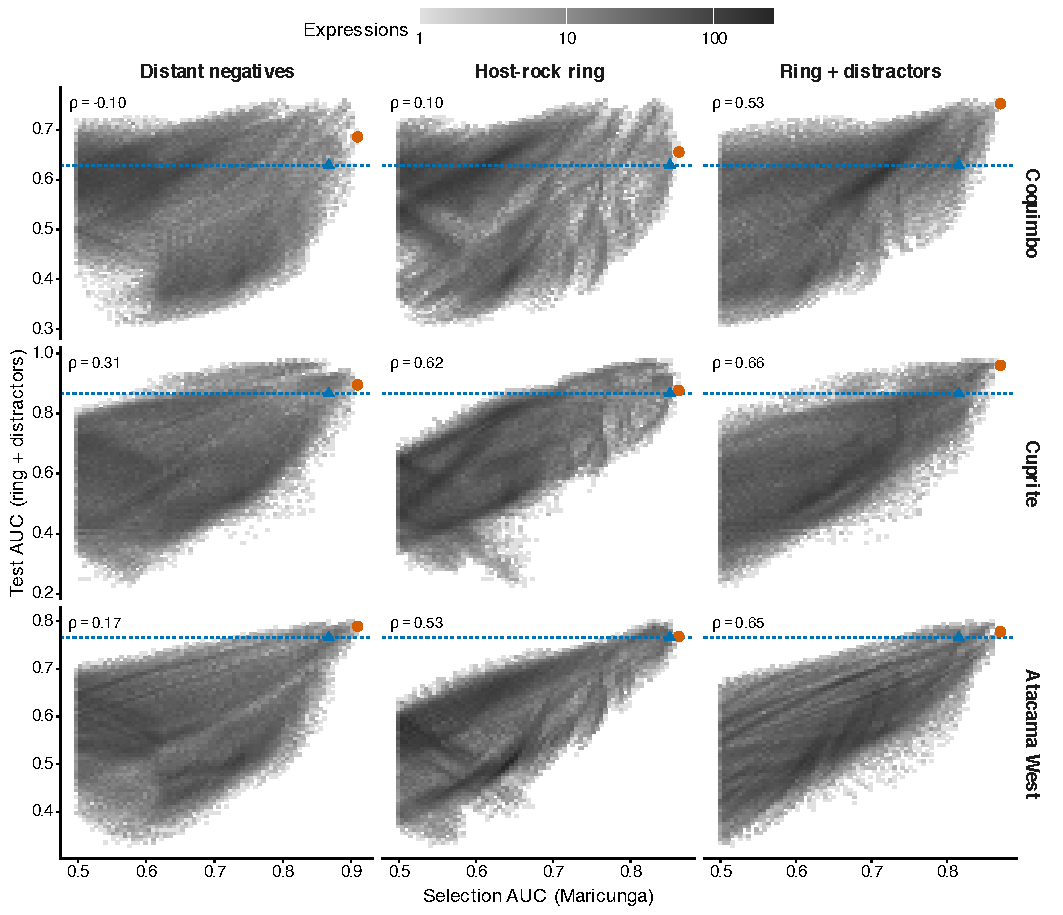
\includegraphics[width=\textwidth]{../figures/v2/fig2_selection_vs_test.pdf}
\caption{Selection AUC in Atacama against test AUC (host-rock ring plus distractors) in Coquimbo (top) and at Cuprite (bottom) for all 87{,}000 expressions with $m \le 4$, under the three selection criteria (columns). Grey shading counts expressions per bin (log scale). Orange circle: winner of each criterion. Blue triangle and dashed line: clay ratio. $\rho$: Spearman correlation between selection and test AUC across the family.}
\label{fig:scatter}
\end{figure*}

\subsection{Exact Pareto front and the selected index}
\label{sec:pareto}

Under the ring-plus-distractors criterion, the selection AUC of the best index rises with complexity from 0.816 (the clay ratio, $m=1$) to 0.846 ($m=2$), 0.857 ($m=3$) and 0.871 ($m=4$) (Fig.~\ref{fig:pareto}). Against the ring plus distractors, the test sites follow the front: Coquimbo AUC is 0.629, 0.701, 0.701 and 0.752, and Cuprite AUC is 0.867, 0.905, 0.913 and 0.960. The fifth factor adds little. The best $m = 5$ index, B02$\cdot$B8A$^3\cdot$B12/(B03$\cdot$B04$\cdot$B06$\cdot$B11$^2$), keeps the structure of the $m = 4$ winner and adds a factor B8A/B06; its selection AUC rises to 0.875, its Coquimbo AUC by 0.010 (0.762) and its Cuprite AUC falls by 0.010 (0.950). We therefore propose the $m = 4$ index and use $m = 5$ as evidence of saturation.

The selected index is not unique in a strong sense. Four expressions lie within 0.005 of its selection AUC, and the runner-up trails by 0.003. All four contain B12/B11 and have B11 squared or cubed in the denominator, combined with a near-infrared term and the blue over green ratio B02/B03 (Section~\ref{sec:physics}). The result to report is this structure, which the next sections interpret, rather than the exact exponents. Within the family, the selected index ranks above the 99.9th percentile in Coquimbo and above the 99.7th at Cuprite; the best expression chosen \emph{a posteriori} on each test set reaches 0.755 in Coquimbo and 0.974 at Cuprite against the ring.

\begin{figure}[ht]
\centering
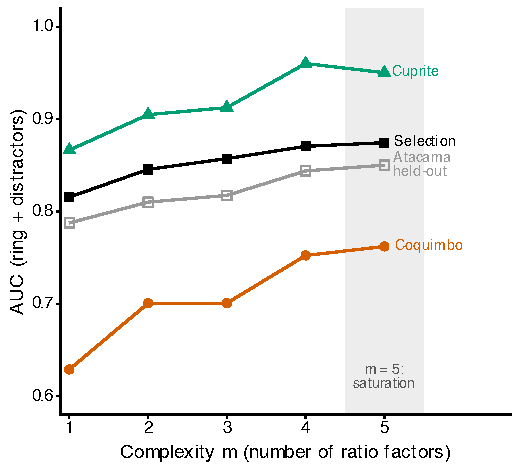
\includegraphics[width=\columnwidth]{../figures/v2/fig3_pareto.pdf}
\caption{Exact Pareto front of the index family under the ring-plus-distractors criterion. For each complexity $m$, the expression with the highest selection AUC is shown with its selection AUC and its AUC against the host-rock ring plus distractors on held-out Atacama pixels, in Coquimbo and at Cuprite. The shaded band marks $m = 5$, where gains stop.}
\label{fig:pareto}
\end{figure}

\subsection{Transfer to Coquimbo and Cuprite}
\label{sec:transfer}

The selected index passes the transfer gate at both test sites (Table~\ref{tab:main}). In Coquimbo it reaches 0.738 AUC against the host-rock ring and 0.752 against the ring plus distractors, against 0.628 and 0.629 for the clay ratio; the gains are 0.110 (95\% block-bootstrap interval 0.042--0.172) and 0.123 (0.066--0.185). At Cuprite it reaches 0.960 in both sets, against 0.903 and 0.867; the gains are 0.057 (0.019--0.109) and 0.094 (0.049--0.158). None of the four intervals includes zero. The mean false-positive rate on distractors falls from 55\% to 10\% in Coquimbo and from 28\% to 5\% at Cuprite. At a fixed false-positive rate of 10\%, the index recovers 43\% of the Coquimbo positives against 27\% for the clay ratio, and 89\% of the Cuprite positives against 66\% (Fig.~\ref{fig:roc}).

In Atacama, on the held-out half, the index reaches 0.844 against the ring plus distractors, against 0.788 for the clay ratio (gain 0.056, interval 0.003--0.119).

\begin{table*}[ht]
\centering
\caption{AUC [95\% block-bootstrap interval] on held-out Atacama pixels and on the two test sites. All indices are oriented and all models trained on the Atacama selection half. Ring = host-rock ring; Hard = ring + distractors.}
\label{tab:main}
\small
\resizebox{\textwidth}{!}{%
\begin{tabular}{lcccccc}
\toprule
 & \multicolumn{2}{c}{Atacama (held-out)} & \multicolumn{2}{c}{Coquimbo} & \multicolumn{2}{c}{Cuprite} \\
 & Ring & Hard & Ring & Hard & Ring & Hard \\
\midrule
Clay ratio B11/B12 & 0.837 & 0.788 & 0.628 & 0.629 & 0.903 & 0.867 \\
Ferric ratio B04/B02 & 0.549 & 0.691 & 0.625 & 0.670 & 0.744 & 0.782 \\
Earlier SR formula $(\sqrt{B12}-B11)^2$ & 0.834 & 0.788 & 0.675 & 0.667 & 0.915 & 0.887 \\
Best $m=2$: B02$\cdot$B12/(B03$\cdot$B11) & 0.810 & 0.810 & 0.672 & 0.701 & 0.925 & 0.905 \\
\textbf{Selected $m=4$ index} & 0.801 & \textbf{0.844} & \textbf{0.738} & \textbf{0.752} & \textbf{0.960} & \textbf{0.960} \\
 & [0.747, 0.844] & [0.802, 0.880] & [0.666, 0.794] & [0.687, 0.806] & [0.942, 0.974] & [0.943, 0.973] \\
Best $m=5$ index & 0.806 & 0.850 & 0.751 & 0.762 & 0.954 & 0.950 \\
\midrule
Logistic, 9 log-ratios & 0.814 & 0.854 & 0.755 & 0.772 & 0.961 & 0.958 \\
Random forest, 10 bands & 0.826 & 0.870 & 0.685 & 0.670 & 0.905 & 0.894 \\
Random forest, 9 log-ratios & 0.822 & 0.881 & 0.660 & 0.662 & 0.880 & 0.885 \\
\bottomrule
\end{tabular}}
\end{table*}

\begin{figure*}[ht]
\centering
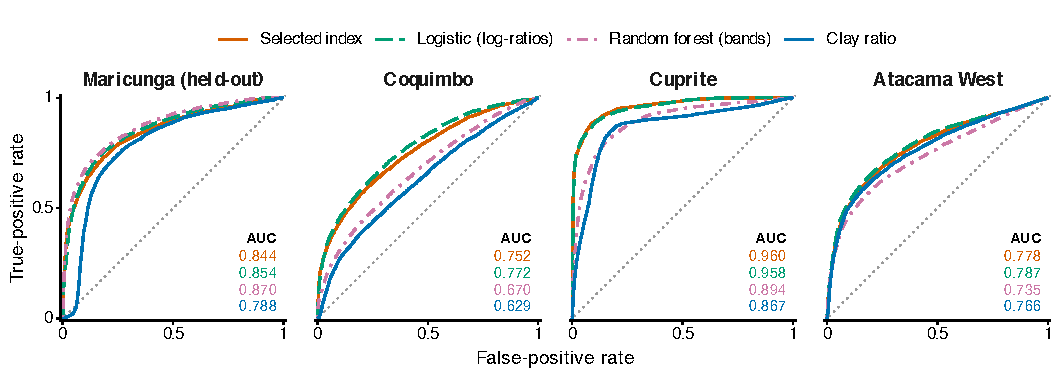
\includegraphics[width=\textwidth]{../figures/v2/fig4_roc.pdf}
\caption{ROC curves against the host-rock ring plus distractors on held-out Atacama pixels, in Coquimbo and at Cuprite, for the selected index, the logistic model on nine log-ratios, a random forest on the ten raw bands and the clay ratio. AUC values are listed in the same colour as each curve; the dotted line is the chance diagonal.}
\label{fig:roc}
\end{figure*}

\subsection{Closed-form index versus models}
\label{sec:models}

A single closed-form index captures almost all the transferable signal of the family. At the test sites the logistic model over all nine log-ratios, which can weight every band freely, exceeds the selected index by 0.017--0.020 in Coquimbo and by at most 0.001 at Cuprite (Table~\ref{tab:main}). The random forests behave differently. On held-out Atacama pixels they are the best classifiers (0.870 and 0.881 against the ring plus distractors), but they lose most of that advantage when moved: in Coquimbo they reach 0.66--0.69, below the selected index and the logistic model, and at Cuprite 0.88--0.91. A flexible model fitted at one site learns more of that site than a constrained index does.

\subsection{RQ3: where the index fails}
\label{sec:failures}

Four results limit the claim. First, against the host-rock ring alone in Atacama, the clay ratio is better than the selected index: 0.837 against 0.801, a difference of 0.036 (interval 0.004--0.065). The selected index wins in Atacama only when distractors are included. Its gain at the selection site therefore comes from rejecting surfaces that mimic alteration, while its gain against host rock appears only at the test sites.

Second, the index fails on some distractors (Fig.~\ref{fig:fpr}). It suppresses vegetation at all sites (false-positive rate 0--1\% against 97--99\% for the clay ratio), shadow in Coquimbo and at Cuprite (10\% and 1\% against 55\% and 60\%) and most salt flats (Uyuni 0\% against 100\%, Maricunga 7\% against 47\%). It still flags 34\% of the Pedernales salt flat (clay ratio 89\%), 30\% of shadow in Atacama (20\%) and 26\% of unaltered alluvium (15\%). At Cuprite it flags 69\% of open-water pixels, against 14\% for the clay ratio. Water is masked in practice, but the index must be used with that mask.

Third, the gain is one of specificity. At the Youden threshold its recall is equal to that of the clay ratio in Atacama (0.73) and lower at the test sites (0.58 against 0.70 in Coquimbo and 0.78 against 0.89 at Cuprite). The higher AUC comes from fewer false positives at a given recall, not from more detections at a fixed threshold.

Fourth, the index is seasonal (Fig.~\ref{fig:temporal}). On the composite of the same season one year earlier it is stable: AUC against the ring plus distractors of 0.843, 0.774 and 0.957 in Atacama, Coquimbo and Cuprite, and Spearman correlations of 0.97, 0.95 and 0.94 with the base composite. On the composite of the opposite season it degrades. In the Atacama winter it falls to 0.726, below the clay ratio (0.764); in the Coquimbo winter to 0.733, still above the clay ratio (0.588); and in the Cuprite spring to 0.903, only 0.025 above the clay ratio (0.878). The Spearman correlation with the base composite drops to 0.75 in Atacama, while that of the clay ratio stays at 0.90.

The selection is also robust to the spatial split. With splits by pixel, by polygon and by \SI{10}{\kilo\meter} blocks, the same index wins and its Coquimbo results are identical. Its held-out Atacama AUC decreases from 0.858 (pixel split) to 0.854 (polygon) and 0.844 (block), and that of the clay ratio decreases by a similar amount (0.803, 0.800, 0.788), so the margin stays between 0.054 and 0.058.

\begin{figure*}[ht]
\centering
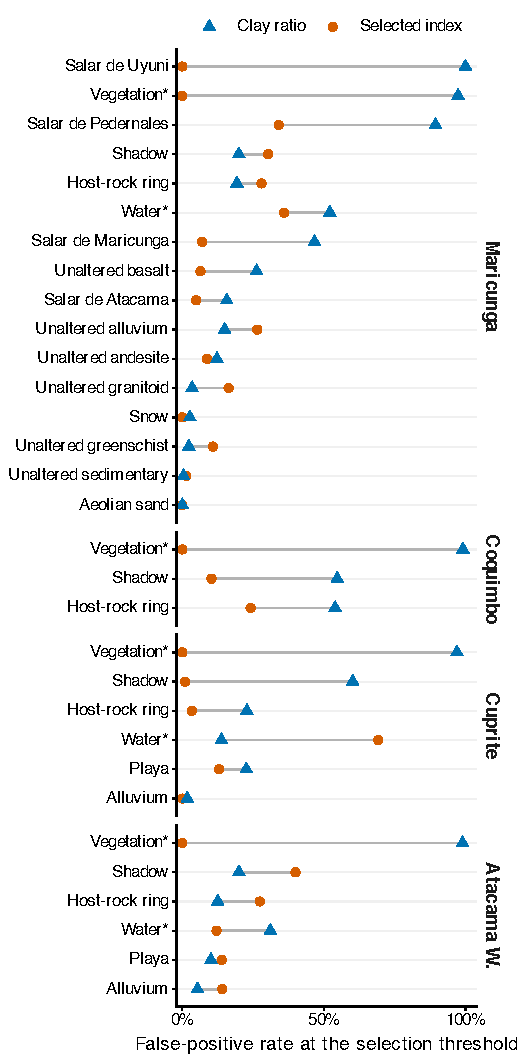
\includegraphics[width=\columnwidth]{../figures/v2/fig5_fpr_groups.pdf}
\caption{False-positive rate of each negative group at the Youden threshold of the selection set, for the selected index (orange circles) and the clay ratio (blue triangles). Atacama groups are the held-out halves. Groups are ordered by the false-positive rate of the clay ratio. Asterisks mark groups masked in practice (vegetation, water), which carry zero weight in selection.}
\label{fig:fpr}
\end{figure*}

\begin{figure*}[ht]
\centering
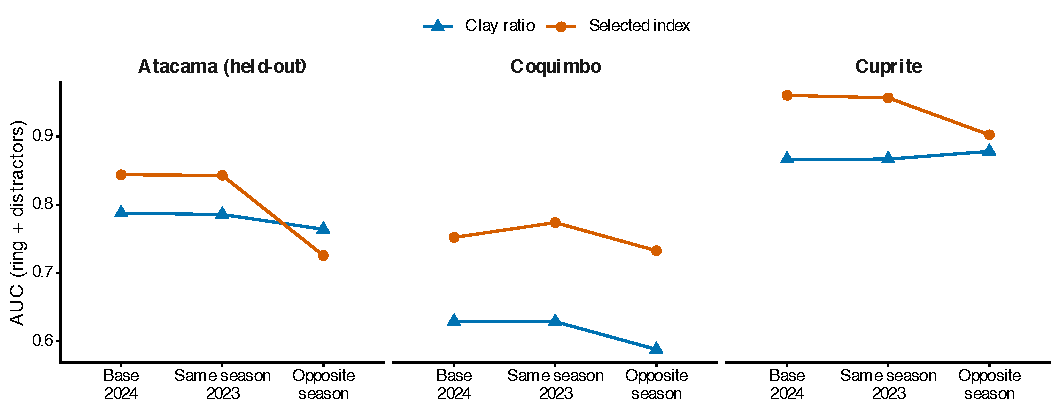
\includegraphics[width=\textwidth]{../figures/v2/fig6_temporal.pdf}
\caption{Temporal stability. AUC against the host-rock ring plus distractors for the selected index and the clay ratio on the base composite (2024 dry season), on the same season one year earlier (2023), and on the opposite season of 2024 (June--September in Chile, March--May at Cuprite). Labels and sets are identical across composites.}
\label{fig:temporal}
\end{figure*}

%% ============================================================
\section{Physical interpretation}
\label{sec:physics}

The selected index is exactly the product of four simple ratios,
\begin{equation}
I = \frac{B02\cdot B8A^{2}\cdot B12}{B03\cdot B04\cdot B11^{2}} = \frac{B12}{B11}\cdot\frac{B8A}{B11}\cdot\frac{B8A}{B04}\cdot\frac{B02}{B03},
\label{eq:decomp}
\end{equation}
and it is oriented so that low values indicate alteration. Table~\ref{tab:terms} gives the median of each factor for altered pixels and for the main negative groups of the Atacama selection set; each factor is lower in altered rock than in the host-rock ring, and each one removes a different set of distractors.

\begin{table}[ht]
\centering
\caption{Median of each factor of Eq.~\ref{eq:decomp} in the Atacama selection set. Low values of $I$ indicate alteration.}
\label{tab:terms}
\begin{tabular}{lrrrrr}
\toprule
Group & B12/B11 & B8A/B11 & B8A/B04 & B02/B03 & $I$ \\
\midrule
Altered (positives) & 0.766 & 0.857 & 1.074 & 0.718 & 0.501 \\
Host-rock ring & 0.914 & 0.931 & 1.103 & 0.762 & 0.709 \\
Alluvium & 0.923 & 0.938 & 1.131 & 0.753 & 0.718 \\
Shadow & 0.912 & 0.976 & 1.065 & 0.805 & 0.728 \\
Salar de Pedernales & 0.712 & 1.076 & 1.067 & 0.839 & 0.682 \\
Salar de Uyuni & 0.543 & 4.310 & 1.001 & 0.966 & 2.314 \\
Snow & 0.996 & 5.726 & 0.872 & 0.992 & 4.706 \\
Vegetation & 0.705 & 1.336 & 2.874 & 0.645 & 1.786 \\
\bottomrule
\end{tabular}
\end{table}

\emph{B12/B11, the inverse of the clay ratio.} Al--OH and Mg--OH bearing minerals (kaolinite, alunite, muscovite, illite, chlorite) absorb between about 2.17 and \SI{2.33}{\micro\meter}, inside the B12 band, while their reflectance at \SI{1.61}{\micro\meter} (B11) stays high \citep{Hunt1977,Clark1999}. The factor is the only one that responds directly to alteration mineralogy, and it separates altered rock from the ring (0.77 against 0.91). It is also low in salt flats and vegetation (0.54--0.71), which is why the clay ratio fires on both.

\emph{B8A/B11.} Near-infrared over the first SWIR band is moderately lower in altered rock than in the ring, but it is very high in snow and in the brightest salt flat (5.7 and 4.3), where reflectance drops between the near infrared and \SI{1.6}{\micro\meter}, and high in vegetation. This factor removes snow and most salt flats.

\emph{B8A/B04.} Near-infrared over red rises steeply in vegetation (2.87 against 1.07) because of the red edge, and it removes vegetation almost completely. Its contrast between altered rock and the ring is small.

\emph{B02/B03.} Blue over green is lowest in altered rock (0.72) and higher in the ring, in shadow, in salt flats and in snow (0.76--0.99). The low value in altered rock is consistent with the charge-transfer absorption of ferric iron in the blue, common where sulfides have weathered to iron oxides \citep{Sabins1999}; the higher values in shadow and evaporites reflect diffuse skylight and flat, bright visible spectra. This factor removes shadow and the remaining salt flats.

Read in this way, the index is the clay ratio corrected by three factors that remove the surfaces on which the clay ratio fails. It explains why the gain is one of specificity (Section~\ref{sec:failures}), and why it degrades in winter: low sun elevation and residual snow change the visible and near-infrared factors more than the SWIR factor, so a SWIR-only index such as the clay ratio is more stable across seasons. We state this last point as an inference; separating illumination and snow effects would require a dedicated experiment.

%% ============================================================
\section{Discussion}
\label{sec:discussion}

\subsection{The negative set as the dominant factor}

The central result is that, with the search held fixed, the choice of negatives decides whether the selected index transfers. Distant negatives produced an index that looked good in Coquimbo for reasons the criterion did not capture, and that failed at Cuprite. Host rock alone produced an index no better than the clay ratio. Only negatives that included the surfaces known to mimic alteration produced an index whose advantage held at both sites. This mirrors what is known about pseudo-absences in species distribution models, where background samples drawn from the wrong environment lead to models that do not transfer \citep{Phillips2009,BarbetMassin2012}, and about negative samples in mineral prospectivity mapping \citep{Zuo2020,Zhang2025}. For spectral indices the practical recommendation is direct: a new index should be reported against the host rock that surrounds the target and against the regional distractors, and at least one site outside the selection area. Gains measured against distant negatives alone should not be taken as evidence of a better alteration index.

\subsection{Enumeration versus stochastic search}

For families of the size used here, enumeration is cheap and removes an uncontrolled source of variation. Scoring every expression up to five ratio factors took about an hour on a laptop, and it made two statements possible that a stochastic search cannot support: that no member of the family scores higher under the criterion, and that the gain from a fifth factor is small. Enumeration does not scale to hyperspectral data, where the number of expressions grows combinatorially with the number of bands; there, stochastic search remains necessary, and its outcome should be compared with exhaustive baselines on smaller problems \citep{Bartlett2024,Kronberger2024}. Our results also suggest a caution for those searches: a better search algorithm cannot compensate for a criterion that rewards the wrong contrast, as Table~\ref{tab:criteria} shows with the same family and three criteria.

\subsection{Why a closed form transfers better than a forest}

The random forests were the best classifiers at the selection site and among the worst at the test sites. We attribute this to inductive bias. Every member of the index family is invariant to multiplicative changes of brightness, and the selected index combines only four ratios with small integer exponents, so it cannot encode much more than spectral shape. A random forest on raw bands can use absolute brightness and site-specific interactions that do not hold elsewhere. Training the forest on log-ratios did not help in Coquimbo (0.66), so scale invariance alone is not sufficient; the constraint on complexity also matters. This explanation is a hypothesis consistent with our results, not a tested mechanism.

\subsection{Limitations}

The Chilean labels limit what any Sentinel-2 index can achieve. In Coquimbo the logistic ceiling is 0.77, while at Cuprite, whose labels come from spectral analysis, the same ceiling is 0.96; much of the remaining error in Chile is probably label noise in 1:100{,}000 polygons rather than a limit of the sensor. The study addresses binary detection of alteration, not the discrimination of alteration types. Selection uses a single site, and the transfer rule was fixed after a pilot in which Coquimbo had been inspected, which makes Cuprite the cleaner test. The index is a dry-season index and must be used with a water mask. Finally, all results come from one sensor; the method applies directly to ASTER and Landsat, but the selected index does not.

\subsection{Transfer of the method}

The negative-set design needs only an alteration map and a composite, and the enumeration needs only the band reflectances, so both can be repeated for other sensors and regions. For ASTER, with nine VNIR--SWIR bands, the family up to $m = 4$ is of similar size to the one enumerated here; for Landsat it is smaller. The code and the extracted pixel tables of the three sites are public, and they allow any new index to be evaluated against the same hard negatives.

%% ============================================================
\section{Conclusions}
\label{sec:conclusions}

With the search held fixed by exhaustive enumeration, the negative set used for selection decided whether a Sentinel-2 alteration index transferred: distant negatives and host rock alone selected indices that failed at independent sites, while host rock plus regional distractors selected one that passed at both. The selected four-ratio index, B02$\cdot$B8A$^2\cdot$B12/(B03$\cdot$B04$\cdot$B11$^2$), outperformed the clay ratio by 0.11--0.12 AUC in Coquimbo and by 0.06--0.09 at Cuprite, came within 0.02 AUC of a logistic model on all log-ratios, and transferred better than random forests trained on the same data. Its advantage is one of specificity against salt flats, shadow and vegetation; it does not beat the clay ratio against host rock alone at the selection site, it fires on open water, and it degrades in the opposite season. We recommend it for dry-season composites with a water mask, and we recommend the hard-negative design as the standard test for any new alteration index.

%% ============================================================
\section*{Data availability}

Sentinel-2 L2A imagery is freely available through the Copernicus programme and Google Earth Engine. The \emph{Atlas Metal\'ifero de la III Regi\'on} and the Coquimbo alteration maps are available from SERNAGEOMIN, and the Cuprite alteration map from the USGS. Code for the negative sampling, the exhaustive enumeration, the baselines and the temporal analysis, together with the extracted pixel tables of the three sites and the per-expression results, is available at \url{https://github.com/franciscoparrao/spectral-indices-discovery}. [Add Zenodo DOI of the archived release.]

\section*{CRediT authorship contribution statement}

\textbf{Francisco Parra~O.}: Conceptualization, Methodology, Software, Validation, Formal analysis, Investigation, Data curation, Writing -- original draft, Writing -- review \& editing, Visualization.
\textbf{Gonzalo R\'ios}: Validation, Writing -- review \& editing.
\textbf{Mauricio Latorre}: Validation, Writing -- review \& editing.

\section*{Declaration of competing interest}

The authors declare that they have no known competing financial interests or personal relationships that could have appeared to influence the work reported in this paper.

\section*{Funding}

This work was supported by MINCIENCIA ANID+ FIUF+ 137139, Fondo de Investigaci\'on Universitaria de Frontera, Vicerrector\'\i a de Investigaci\'on, Innovaci\'on y Creaci\'on, Universidad de Santiago de Chile. M.L.\ was supported by ANID Anillo Regular ACT210004; ANID Apoyo a Centros de Excelencia ACE210010 (Center for Mathematical Modeling); ANID Millennium Science Initiative Program ICN2021\_044; Fondo Basal FB210005; and ANID FONDECYT 1230194. The funders had no role in study design, in the collection, analysis and interpretation of data, in the writing of the report, or in the decision to submit the article for publication.

\section*{Declaration of generative AI and AI-assisted technologies in the manuscript preparation process}

During the preparation of this work the authors used Claude (Anthropic) to assist with code development for the analysis pipeline and to generate a first draft of the manuscript text from the authors' results and outline. After using this tool, the authors reviewed and edited the content as needed and take full responsibility for the content of the published article.

\section*{Acknowledgements}

The authors acknowledge SERNAGEOMIN for making the \emph{Atlas Metal\'ifero de la III Regi\'on} and the regional alteration maps publicly available, and the USGS for the alteration map of the southwestern United States \citep{Rockwell2017}.

\bibliographystyle{elsarticle-harv}
\bibliography{references_v2}

\end{document}
